\documentclass[9pt,aspectratio=169,xcolor=table]{beamer}

%~~~~~~~~~~~~~~~~~~~~~~~~~~~~~~~~~~~~~~~~~~~~~~~~~~~~~~~~~~~~~~~~~~~~~~~~~~~~~~
% Use roboto Font (recommended)
\usepackage[sfdefault]{roboto}
\usepackage[utf8]{inputenc}
\usepackage[T1]{fontenc}
%~~~~~~~~~~~~~~~~~~~~~~~~~~~~~~~~~~~~~~~~~~~~~~~~~~~~~~~~~~~~~~~~~~~~~~~~~~~~~~

%~~~~~~~~~~~~~~~~~~~~~~~~~~~~~~~~~~~~~~~~~~~~~~~~~~~~~~~~~~~~~~~~~~~~~~~~~~~~~~
% Define where theme files are located. ('/styles')
\usepackage{styles/fluxmacros}
\usefolder{styles}
% Use Flux theme v0.1 beta
% Available style: asphalt, blue, red, green, gray
\usetheme[style=gray]{flux}
%~~~~~~~~~~~~~~~~~~~~~~~~~~~~~~~~~~~~~~~~~~~~~~~~~~~~~~~~~~~~~~~~~~~~~~~~~~~~~~

%~~~~~~~~~~~~~~~~~~~~~~~~~~~~~~~~~~~~~~~~~~~~~~~~~~~~~~~~~~~~~~~~~~~~~~~~~~~~~~
% Extra packages
\usepackage{booktabs}
\usepackage{colortbl}
\usepackage{ragged2e}
\usepackage{amssymb}
\usepackage{multirow}
\usepackage{tikz}
\usetikzlibrary{arrows.meta, positioning, fit, backgrounds, calc, decorations.pathreplacing}
\setbeamertemplate{itemize items}[square]
\usepackage[scaled=.92]{beramono}
\usepackage{listings}
\usepackage{styles/lstlangarm}
\usepackage{array}
\definecolor{bgcolor}{HTML}{F2E9E9}
% lstlangarm.sty references \color{mauve} for string literals but never defines
% it -- only fires when a listing contains a string. Define it here.
\definecolor{mauve}{rgb}{0.58,0,0.82}
% lstlangarm's C style sets commentstyle=green!20, which is unreadable on the
% pink listing background. Darken it globally.
\lstset{commentstyle=\color{green!45!black}}
% ragged-right fixed-width column -- must be defined in the preamble, never
% inside a frame (\newcolumntype's #1 breaks beamer's frame scanner)
\newcolumntype{R}[1]{>{\RaggedRight\arraybackslash}p{#1}}
%~~~~~~~~~~~~~~~~~~~~~~~~~~~~~~~~~~~~~~~~~~~~~~~~~~~~~~~~~~~~~~~~~~~~~~~~~~~~~~
% Table striping: odd rows white, even rows very light gray.
% Needs \documentclass[...,xcolor=table]{beamer} (beamer loads xcolor itself,
% so the option must go on the class, not \usepackage).
\definecolor{stripe}{gray}{0.94}
% \striped makes body rows alternate white, gray, white, ... starting white.
% \rowcolors counts from the first coloured body row; the header is not counted.
\newcommand{\striped}{\rowcolors{1}{white}{stripe}}
%~~~~~~~~~~~~~~~~~~~~~~~~~~~~~~~~~~~~~~~~~~~~~~~~~~~~~~~~~~~~~~~~~~~~~~~~~~~~~~

%~~~~~~~~~~~~~~~~~~~~~~~~~~~~~~~~~~~~~~~~~~~~~~~~~~~~~~~~~~~~~~~~~~~~~~~~~~~~~~
% TikZ block styles -- matches ch1/ch2
% Colour variables are named identically in the book's stm32primer.tex, so any
% tikzpicture using only the \tikzset{...} styles below can be copied verbatim
% between slides and book. Only the \definecolor/\colorlet VALUES differ: the
% book is printed, so it keeps every stroke pure black with muted fills. These
% slides are projected, so both fill AND stroke are bright and saturated to
% grab attention -- see stm32primer.tex for the print palette.
\definecolor{blkfill}{HTML}{DCEBFF}
\definecolor{blkline}{HTML}{1565C0}
\definecolor{accentfill}{HTML}{FFE0B2}
\definecolor{accentline}{HTML}{E65100}
\definecolor{memfill}{HTML}{DFF5DA}
\definecolor{memline}{HTML}{2E7D32}
\definecolor{cellfill}{HTML}{FFFFFF}
\definecolor{cellline}{HTML}{424242}
\definecolor{bitmaskfill}{HTML}{DCEBFF}
\definecolor{bitmaskline}{HTML}{1565C0}
\definecolor{bithitfill}{HTML}{FFE0B2}
\definecolor{bithitline}{HTML}{E65100}
\tikzset{
  blk/.style   = {rectangle, rounded corners=2pt, draw=blkline, fill=blkfill,
                  thick, align=center, font=\small, minimum height=9mm, inner sep=3pt},
  cpublk/.style= {rectangle, rounded corners=2pt, draw=accentline, fill=accentfill,
                  thick, align=center, font=\small\bfseries, minimum height=9mm, inner sep=3pt},
  memblk/.style= {rectangle, rounded corners=2pt, draw=memline, fill=memfill,
                  thick, align=center, font=\small, minimum height=9mm, inner sep=3pt},
  cell/.style  = {rectangle, draw=cellline, fill=cellfill, align=center,
                  font=\normalsize\ttfamily, minimum height=7mm, inner sep=2pt},
  lbl/.style   = {font=\scriptsize, text=Gray},
  flow/.style  = {-{Stealth[length=2mm]}, thick, draw=blkline},
  busline/.style={thick, draw=cellline},
}
% NOTE (theme quirks -- always page through the PDF; most fail silently,
% but the \\ one below is a FATAL cascade, not silent):
%  - a second \\ inside a nested {...} group in a TikZ node breaks parsing
%  - TWO OR MORE \\ line breaks in a single plain TikZ \node label ALSO
%    breaks parsing, even with no nested group -- this is fatal (a ~40-error
%    cascade ending "Missing \begin{document}"), not silent. Keep node labels
%    to at most one \\; for more lines use align=left/center plus a comma or
%    "and" instead of a second break, or accept the one-\\ limit.
%  - a bare pgfmath expression {a - b*c} used directly as a coordinate
%    component (e.g. "at (x,{expr})") can also misparse in LR mode inside a
%    node -- precompute it with \pgfmathsetmacro{\name}{expr} first and use
%    \name in the coordinate instead
%  - text placed directly after \begin{frame}{Title} on the very next line
%    (e.g. an immediate {\small ...} paragraph) can get swallowed into the
%    title, leaving the title bar BLANK -- prefix the body with \leavevmode
%  - {\small ...} wrapped around a nested itemize eats the frame title + list
%  - \usebeamercolor on a [plain] frame falls through to an unstyled default
%  - \newcolumntype inside a frame breaks beamer's frame scanner
%  - lstlisting needs \begin{frame}[fragile]
%  - a TikZ picture wider than its column silently overflows into neighbours
%~~~~~~~~~~~~~~~~~~~~~~~~~~~~~~~~~~~~~~~~~~~~~~~~~~~~~~~~~~~~~~~~~~~~~~~~~~~~~~

%%%%%%%%%%%%%%%%%%%%%%%%%%%%%%%%%%%
%% BEGIN CONDITIONAL COMPILATION %%
%%%%%%%%%%%%%%%%%%%%%%%%%%%%%%%%%%%
\newif\ifwebex
%\webextrue % uncomment to generate section separator
\ifwebex
\AtBeginSection[]{
  \begin{frame}
  \vfill
  \centering
  \begin{beamercolorbox}[sep=8pt,center,shadow=true,rounded=true]{title}
    \usebeamerfont{title}\insertsectionhead\par%
  \end{beamercolorbox}
  \vfill
  \end{frame}
}
\else
\AtBeginSection[]
{
{
    \setbeamercolor{background canvas}{bg=yellow!10}
    \begin{frame}[plain]
        \frametitle{Table of Contents}
        \tableofcontents[currentsection]
    \end{frame}
}
}
\fi
%%%%%%%%%%%%%%%%%%%%%%%%%%%%%%%%%%%
%% END CONDITIONAL COMPILATION   %%
%%%%%%%%%%%%%%%%%%%%%%%%%%%%%%%%%%%

%~~~~~~~~~~~~~~~~~~~~~~~~~~~~~~~~~~~~~~~~~~~~~~~~~~~~~~~~~~~~~~~~~~~~~~~~~~~~~~
% Information
\title{Interrupts and Event-Driven Programming}
\subtitle{\emph{Introduction to ARM Cortex-M Microprocessors} --- Chapter 9}
\author{Mun\'{i}m Zabidi}
\institute{\color{primary}Faculty of Electrical Engineering, Universiti Teknologi Malaysia}
\date{\today}
\titlegraphic{assets/logoutmwhite.png}
%~~~~~~~~~~~~~~~~~~~~~~~~~~~~~~~~~~~~~~~~~~~~~~~~~~~~~~~~~~~~~~~~~~~~~~~~~~~~~~

\begin{document}

\titlepage

\begin{frame}{Table of Contents}
    \tableofcontents
\end{frame}

%===============================================================================
\section{Why This Matters}
%===============================================================================

\begin{frame}{Why This Chapter Matters}
    \leavevmode
    Experiment 6 in the previous chapter measured reaction time. It sat in a loop and read a button. While it waited, the processor could do nothing else --- no display update, no sensor reading, no communication. Worse, it could not sleep. A battery-powered version would drain continuously while waiting for an event that might be minutes away. Polling does not scale. This chapter introduces a better mechanism: hardware that interrupts the processor when something actually happens. This is how every real embedded system is built. We will trace one concrete event --- a press of the PC13 button --- from the pin to the line of C code that responds to it. That single trace introduces every piece of the architecture along the way.
\end{frame}

\begin{frame}{Objectives}
    \leavevmode
    {\small After completing this chapter, you should be able to:}

    \vspace{2mm}
    {\small
    \begin{enumerate}\itemsep2pt
        \item Contrast the polling and interrupt models and justify the choice of each.
        \item Explain the role of the vector table and how the NVIC dispatches an interrupt.
        \item Describe the sequence of events from an external pin change to the execution of an ISR.
        \item Configure the EXTI controller and SYSCFG to route a GPIO pin to an interrupt line.
        \item Write an ISR that correctly clears its pending flag and shares data with the main program.
        \item Use interrupt priorities and masking registers to control preemption.
    \end{enumerate}}
\end{frame}


%===============================================================================
\section{Polling and Interrupts}
%===============================================================================
\begin{frame}[fragile]{Polling and Interrupts}
	\begin{columns}[T]
		\begin{column}{.48\textwidth}
			\textbf{Polling}

			\vspace{1mm}
			\begin{lstlisting}[style=myc, basicstyle=\ttfamily\small]
while (1) {
	if (button_pressed())
		do_something();
}
			\end{lstlisting}

			\vspace{5mm}
			{\small
				\begin{itemize}\itemsep1pt
					\item The processor \alert{repeatedly checks} for the event
					\item Simple to write and understand
					\item Processor time is spent checking even when nothing happens
					\item Response time depends on how often the event is checked
			\end{itemize}}
		\end{column}

		\begin{column}{.48\textwidth}
			\textbf{Interrupts}

			\vspace{1mm}
			\begin{lstlisting}[style=myc, basicstyle=\ttfamily\small]
void EXTI15_10_IRQHandler(void) {
	do_something();
}
			\end{lstlisting}

			\vspace{5mm}
			{\small
				\begin{itemize}\itemsep1pt
					\item Hardware signals the processor when the event occurs
					\item The processor can sleep or do other work meanwhile
					\item Response does not depend on continuously checking the event
			\end{itemize}}
		\end{column}
	\end{columns}

	\vspace{3mm}
	\begin{block}{The key difference}
		\alert{Polling asks ``Has it happened yet?'' repeatedly.}
		An interrupt lets the hardware say ``It has happened.''
	\end{block}
\end{frame}

\begin{frame}{Interrupts vs.\ Polling, on the Wire}
    \leavevmode
    \definecolor{cpugreen}{RGB}{110,190,40}
    \definecolor{gpioblue}{RGB}{50,120,190}
    \definecolor{cpured}{RGB}{200,30,30}
    \definecolor{purp}{RGB}{110,50,150}
    \definecolor{dgray}{RGB}{125,130,135}
    \definecolor{lgray}{RGB}{200,200,205}

    \begin{center}
    \resizebox{.8\textwidth}{!}{%
    \begin{tikzpicture}[x=0.022cm, y=-0.022cm, font=\footnotesize,
      chip/.style={rounded corners=2pt, text=white, font=\footnotesize\bfseries,
                   minimum width=1.0cm, minimum height=0.65cm, inner sep=0pt},
      darr/.style={dashed, dash pattern=on 2pt off 2pt, -{Stealth[length=4pt]}, dgray}]

      % ---------- vertical event line ----------
      \draw[purp, line width=0.7pt] (432,8) -- (432,296);

      % ================= POLLING (top) =================
      \begin{scope}[shift={(0,-136)}]
        \node[align=center] at (50,190) {When\\Using\\Polling};
        \node[chip, fill=cpugreen] at (102,180) {CPU};
        \node[chip, fill=gpioblue] at (102,243) {GPIO};

        \draw[cpugreen, line width=6pt, line cap=butt]
          (125,180) -- (193,180) (222,180) -- (293,180) (322,180) -- (393,180)
          (422,180) -- (492,180);
        \draw[cpured, line width=6pt, line cap=butt] (521,180) -- (680,180);
        \draw[cpugreen, line width=1.2pt, line cap=butt]
          (193,180) -- (222,180) (293,180) -- (322,180)
          (393,180) -- (422,180) (492,180) -- (521,180);
        \draw[gpioblue, line width=1.2pt] (125,243) -- (680,243);

        \foreach \x in {193,293,393,492}{
          \fill[dgray] (\x,233) rectangle (\x+29,253);
          \draw[darr] (\x,183)    -- (\x,233);
          \draw[darr] (\x+29,233) -- (\x+29,183);
        }
        \foreach \x in {158,258,358,458}{
          \node at (\x,210) {Check state};
        }

        \node[anchor=west, align=left] at (521,158)
          {Perform processing in\\response to state change};
      \end{scope}

      % ================= INTERRUPTS (bottom) =================
      \begin{scope}[shift={(0,136)}]
        \node[align=center] at (50,78) {When\\Using\\Interrupts};
        \node[chip, fill=cpugreen] at (102,46)  {CPU};
        \node[chip, fill=gpioblue] at (102,110) {GPIO};

        \draw[cpured, line width=1.2pt] (125,46) -- (447,46);
        \draw[cpured, line width=6pt, line cap=butt] (447,46) -- (680,46);
        \draw[gpioblue, line width=1.2pt] (125,110) -- (680,110);

        \fill[dgray] (432,100) rectangle (447,120);
        \draw[darr] (447,100) -- (447,51);
        \node[anchor=west] at (452,80) {Throw interrupt};
        \node[anchor=west, align=left] at (452,22)
          {Perform processing in\\response to interrupt event};
      \end{scope}

      % callout
      \node[draw, fill=white, anchor=west, inner sep=3pt] (c) at (140,290)
        {GPIO input value change from 0 to 1};
      \draw[-{Stealth[length=4pt]}] (c.east) -- (430,290);
    \end{tikzpicture}}
    \end{center}

    {\footnotesize \begin{itemize}
    		\item With
    		polling, the CPU keeps checking the state, whether or not anything
    		has changed. It only notices a change on its next check.
    		\item With interrupts, the CPU does nothing until the GPIO line
    		actually changes --- \alert{one} response, exactly when needed.
    	\end{itemize} }
\end{frame}

\begin{frame}{When Should I Use Each?}
	\leavevmode
	{\small Both methods exist for good reasons. The real question is not
		\alert{which is better}, but \alert{what the code needs to ask}: ``is
		this true right now?'' (polling), or ``tell me when this becomes
		true'' (interrupt).}

	\begin{center}
		{\small
			\striped
			\begin{tabular}{@{}l l l@{}}
				\toprule
				\textbf{Decision factor} & \textbf{Favours interrupts} & \textbf{Favours polling} \\
				\midrule
				Timing of the event & Asynchronous, unpredictable & Periodic, or always true \\
				Response deadline & Latency-sensitive & Non-critical \\
				Power budget & Must sleep between events & Actively running anyway \\
				Setup cost & Worth the NVIC/EXTI setup & A checking loop is enough \\
				\bottomrule
		\end{tabular}}
	\end{center}

	{\small A button press happens at random times and needs a fast
		response, so \alert{interrupts win}. A sensor you already read every
		loop pass needs nothing extra, so \alert{polling is simplest}.}
\end{frame}

\begin{frame}{What Happens When an Interrupt Fires}
    \leavevmode
    {\scriptsize We use an \alert{external} interrupt: a button
    on a pin. %The same NVIC and vector-table mechanism also handles
%    \alert{inte%rnal peripheral} events (timer, UART) and
%    \alert{softw%are or exception} events (a fault, or a manual trigger).
%    Back to the button:
    }

    \begin{columns}[c]
    \begin{column}{.52\textwidth}
        \begin{center}
        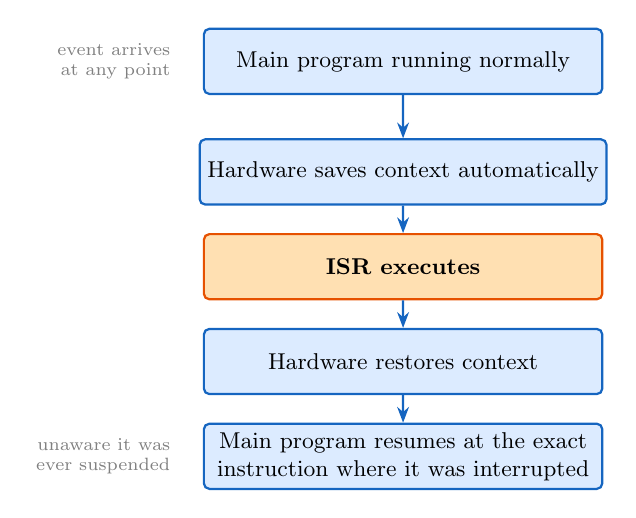
\begin{tikzpicture}[node distance=3.5mm, every node/.style={scale=0.92}]
            \node[blk, minimum width=55mm] (run)  {Main program running normally};
            \node[blk, below=5.5mm of run, minimum width=55mm, font=\small]
                 (save) {Hardware saves context automatically};
            \node[cpublk, below=of save, minimum width=55mm] (isr)  {ISR executes};
            \node[blk, below=of isr,  minimum width=55mm] (rest) {Hardware restores context};
            \node[blk, below=of rest, minimum width=55mm, align=center]
                 (res)  {Main program resumes at the exact\\instruction where it was interrupted};

            \draw[flow] (run)  -- (save);
            \draw[flow] (save) -- (isr);
            \draw[flow] (isr)  -- (rest);
            \draw[flow] (rest) -- (res);

            \node[lbl, anchor=east, font=\scriptsize, align=right,
                  left=3mm of run.west] {\alert{event arrives}\\at any point};
            \node[lbl, anchor=east, font=\scriptsize, align=right,
                  left=3mm of res.west] {unaware it was\\ever suspended};
        \end{tikzpicture}
        \end{center}
    \end{column}
    \begin{column}{.44\textwidth}
        The processor saves this context \alert{for you}, in hardware,
        before your handler runs.

        \vspace{3mm}
        \begin{block}{Chapter 7's stack, used automatically}
            It pushes \texttt{R0--R3}, \texttt{R12}, \texttt{LR}, \texttt{PC} and
            \texttt{xPSR} --- \alert{eight words} --- and pops them back on return.

            \vspace{2mm}
            Your interrupted code never notices this happened.
        \end{block}

        \vspace{2mm}
        {\small These eight are the \alert{caller-saved} registers from the AAPCS.
        Your handler must save anything else it uses --- the C compiler
        does this automatically.}
    \end{column}
    \end{columns}
\end{frame}

\begin{frame}{The Same Interrupt, Viewed Against Time}
    \leavevmode
    \begin{center}
    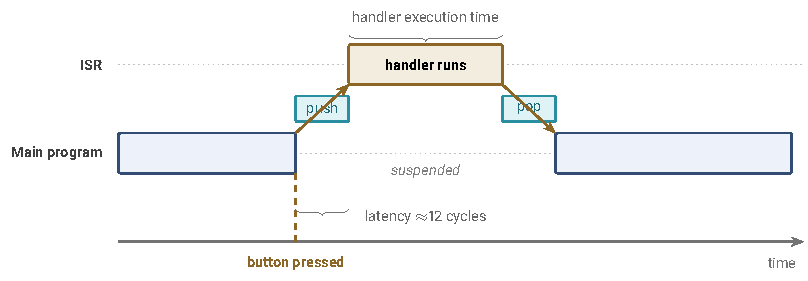
\includegraphics[width=.92\textwidth]{assets/isr-timing.pdf}
    \end{center}

    \vspace{1mm}
    {\small Only one row runs at any instant. The main program is
    \alert{paused} for the whole shaded span, then resumes at the exact
    instruction it was about to run. Two numbers matter here: the
    \alert{latency} before the handler starts, and the handler's own
    \alert{execution time} --- how long the main program must wait.}
\end{frame}

%===============================================================================
\section{The Vector Table and NVIC}
%===============================================================================

\begin{frame}{Who Routes the Event?}
    \leavevmode
    {\small You have seen the event happen, and what the hardware does
    around it. One question is still open: \alert{how does the processor
    know which function to call?} The answer is a chain of five links.
    This section, and the next, explain the middle three.}

    \vspace{4mm}
    \begin{center}
    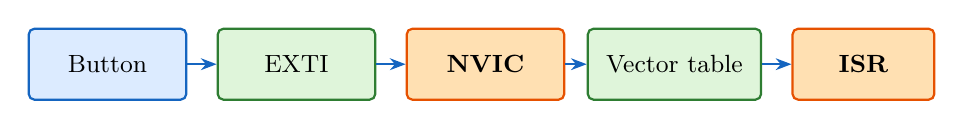
\begin{tikzpicture}[x=24mm, y=10mm]
        \node[blk,    minimum width=20mm] (btn) at (0,0) {Button};
        \node[memblk, minimum width=20mm] (ext) at (1,0) {EXTI};
        \node[cpublk, minimum width=20mm] (nvi) at (2,0) {NVIC};
        \node[memblk, minimum width=22mm] (vec) at (3,0) {Vector table};
        \node[cpublk, minimum width=18mm] (isr) at (4,0) {ISR};
        \foreach \x/\y in {btn/ext, ext/nvi, nvi/vec, vec/isr}{\draw[flow] (\x) -- (\y);}
    \end{tikzpicture}
    \end{center}

    \vspace{4mm}

{\small
	\begin{enumerate}
		\item \alert{EXTI} notices the pin change.
		\item The \alert{NVIC} looks at all pending interrupts and picks a winner.
		\item The \alert{vector table} says where that winner's code lives.
		\item The processor jumps there.
		\item Every interrupt uses these same five links, no matter its source.
	\end{enumerate}
	}\end{frame}

\begin{frame}{The Vector Table}
    \begin{columns}[T]
    \begin{column}{.5\textwidth}
        A table at the \alert{start of flash memory}. It holds the
        address of every handler.

        \vspace{2mm}
        {%
        \striped
        \begin{tabular}{@{}l l@{}}
            \toprule
            \textbf{Offset} & \textbf{Contains} \\
            \midrule
            \texttt{0x00} & Initial \texttt{SP} value \\
            \texttt{0x04} & Reset handler \\
            \texttt{0x08} & NMI handler \\
            \texttt{0x0C} & HardFault handler \\
            \ldots        & \ldots \\
            \texttt{0x3C} & SysTick handler \\
            \texttt{0x40}+ & The device interrupts \\
            \bottomrule
        \end{tabular}}
    \end{column}
    \begin{column}{.46\textwidth}
        \begin{block}{Where the initial SP comes from}
            The \alert{first word} holds the starting stack pointer. The
            hardware loads this automatically at reset, before a single
            instruction runs.
        \end{block}

        \vspace{2mm}
        {\small When an interrupt fires, the processor looks up its handler
        here and jumps to it. This is why your handler must have
        \alert{exactly the right name}. The startup file maps that name
        into the table.}
    \end{column}
    \end{columns}
\end{frame}

\begin{frame}{Reading the Vector Table}
    \leavevmode
    \begin{center}
    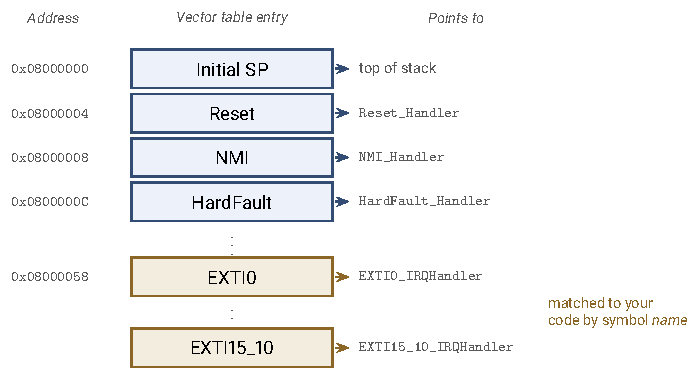
\includegraphics[height=.6\textheight]{assets/vector-table.pdf}
    \end{center}

    {\small Two things follow from this. First, the linker matches your
    handler to a slot by \alert{symbol name}. Misspell it, and a silent
    do-nothing handler runs instead of yours. Second, every entry's low
    bit is set to 1 to select Thumb state --- this is why handler
    addresses look odd in a debugger.}
\end{frame}

\begin{frame}{Where the NVIC Sits}
    \leavevmode
    \begin{center}
    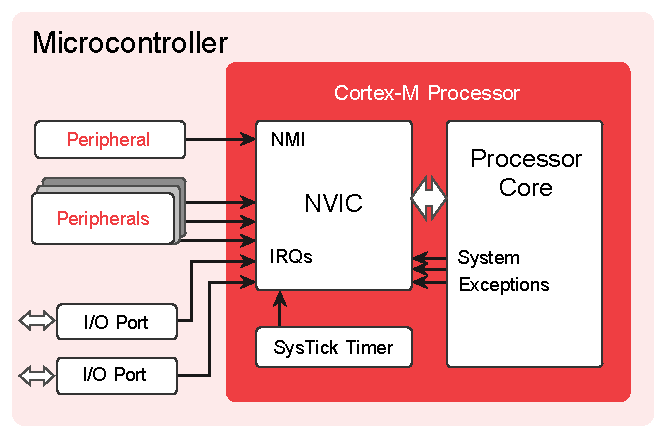
\includegraphics[height=.6\textheight]{assets/nvic.pdf}
    \end{center}

    {\small Every interrupt source feeds into the NVIC: external
    peripherals, I/O ports, the \alert{SysTick timer}, even an
    \texttt{NMI}. The NVIC picks exactly one at a time and hands it to
    the \alert{Processor Core}, alongside the core's own \alert{system
    exceptions} (HardFault and the rest).}
\end{frame}

\begin{frame}{The NVIC}{Nested Vectored Interrupt Controller}
    \begin{columns}[T]
    \begin{column}{.5\textwidth}
        {\small
        \striped
        \begin{tabular}{@{}l l@{}}
            \toprule
            \textbf{CMSIS function} & \textbf{Does} \\
            \midrule
            \texttt{NVIC\_EnableIRQ(n)}     & Enable interrupt \texttt{n} \\
            \texttt{NVIC\_DisableIRQ(n)}    & Disable it \\
            \texttt{NVIC\_SetPriority(n,p)} & Set its priority \\
            \bottomrule
        \end{tabular}}

        \vspace{3mm}
        {\small \alert{Nested} means a higher-priority interrupt can
        interrupt a handler that is already running.

        \alert{Vectored} means the hardware jumps straight to the right
        handler. There is no software dispatch step.}
    \end{column}
    \begin{column}{.46\textwidth}
        \begin{block}{Lower number means higher priority}
            Priority \texttt{0} is the most urgent. This feels backwards
            at first, and it is a common source of bugs.
        \end{block}

        \vspace{2mm}
        {\small \texttt{\_\_disable\_irq()} and \texttt{\_\_enable\_irq()} mark
        a \alert{critical section}: a piece of code that must not be
        interrupted once it starts.}
    \end{column}
    \end{columns}
\end{frame}

%===============================================================================
\section{Handling External Interrupts}
%===============================================================================

\begin{frame}{From Pin to Handler}
    \begin{center}
    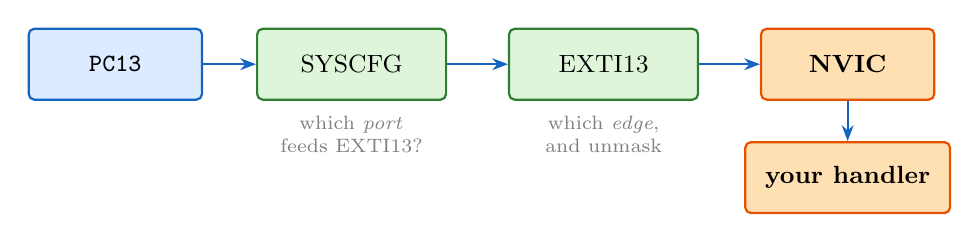
\begin{tikzpicture}[x=10mm, y=9mm]
        \node[blk,    minimum width=22mm] (p) at (0,0)   {\texttt{PC13}};
        \node[memblk, minimum width=24mm] (s) at (3.0,0) {SYSCFG};
        \node[memblk, minimum width=24mm] (e) at (6.2,0) {EXTI13};
        \node[cpublk, minimum width=22mm] (n) at (9.3,0) {NVIC};
        \node[cpublk, minimum width=26mm] (h) at (9.3,-1.6) {your handler};
        \foreach \x/\y in {p/s, s/e, e/n}{\draw[flow] (\x) -- (\y);}
        \draw[flow] (n) -- (h);
        \node[lbl, anchor=north, align=center] at (3.0,-0.6) {which \emph{port}\\feeds EXTI13?};
        \node[lbl, anchor=north, align=center] at (6.2,-0.6) {which \emph{edge},\\and unmask};
    \end{tikzpicture}
    \end{center}

    \vspace{3mm}
    \begin{block}{Four things to configure, in order: Route, Trigger, Enable, Handle}
        \begin{enumerate}
            \item \textbf{Route} (\textbf{SYSCFG}) --- choose which port's pin 13
                  drives EXTI13
            \item \textbf{Trigger} (\textbf{EXTI}) --- select the trigger edge,
                  then unmask the line
            \item \textbf{Enable} (\textbf{NVIC}) --- enable the interrupt and set
                  its priority
            \item \textbf{Handle} --- write the handler, with the name the vector
                  table expects
        \end{enumerate}
    \end{block}
\end{frame}

\begin{frame}[plain]{EXTI Lines Are Shared}
    \begin{columns}[c]
    \begin{column}{.4\textwidth}
        \begin{center}
        \includegraphics[height=.82\textheight, keepaspectratio]%
            {assets/exti-mapping.png}
        \end{center}
    \end{column}
    \begin{column}{.56\textwidth}
        All \texttt{Px0} pins feed \texttt{EXTI0}. All \texttt{Px1} pins
        feed \texttt{EXTI1}, and so on. But \alert{only one} pin per number
        can be selected at a time.

        \vspace{3mm}
        \begin{block}{A design constraint, not a small detail}
            You cannot have \texttt{PA0} \emph{and} \texttt{PB0} both
            generating interrupts at the same time.

            \vspace{2mm}
            Interrupt-capable inputs must use \alert{different pin
            numbers}. This is a pin-assignment decision you make on
            paper, before the board is built.
        \end{block}

        \vspace{3mm}
        {\small \texttt{SYSCFG->EXTICR[x]} chooses which port drives each
        line: four bits per line, four lines per register.}
    \end{column}
    \end{columns}
\end{frame}

\begin{frame}[fragile]{The Configuration Sequence}
\begin{lstlisting}[style=myc, basicstyle=\ttfamily\small, numbers=left]
// 0. Clocks
RCC->AHB1ENR |= (1U << 2);        // GPIOC
RCC->APB2ENR |= (1U << 14);       // SYSCFG

// 1. ROUTE: PC13 to EXTI13  (EXTICR[3], bits 7:4, value 0010 = port C)
SYSCFG->EXTICR[3] &= ~(0xFU << 4);
SYSCFG->EXTICR[3] |=  (0x2U << 4);

// 2. TRIGGER: falling edge -- an active-low button goes HIGH->LOW
EXTI->FTSR |= (1U << 13);
EXTI->IMR  |= (1U << 13);         // unmask the line

// 3. ENABLE in the NVIC
NVIC_SetPriority(EXTI15_10_IRQn, 2);
NVIC_EnableIRQ(EXTI15_10_IRQn);

// 4. HANDLE: write EXTI15_10_IRQHandler -- next section
\end{lstlisting}

    \vspace{1mm}
    {\small Lines 10--15 all share one handler,
    \texttt{EXTI15\_10\_IRQHandler}. This is why the handler must check
    \emph{which} line fired.}
\end{frame}

%===============================================================================
\section{Writing a Handler}
%===============================================================================

\begin{frame}[fragile]{The Handler}
\begin{lstlisting}[style=myc, basicstyle=\ttfamily\small]
volatile uint8_t button_event = 0;     // shared with main() -> volatile

void EXTI15_10_IRQHandler(void)
{
    if (EXTI->PR & (1U << 13)) {       // was it line 13?
        EXTI->PR = (1U << 13);         // clear it by writing 1
        button_event = 1;              // just record it; main() acts
    }
}
\end{lstlisting}

    \vspace{5mm}
    \begin{block}{Three rules, and each one matters}
        \begin{enumerate}
            \item The \alert{name} must match the vector table exactly.
            \item \alert{Clear the pending flag}, by writing \texttt{1} to
                  it. Skip this, and the handler runs forever.
            \item Anything shared with \texttt{main()} must be
                  \alert{\texttt{volatile}}.
        \end{enumerate}
    \end{block}
\end{frame}

\begin{frame}{Sharing Data With an ISR}
    \begin{columns}[T]
    \begin{column}{.48\textwidth}
        \textbf{Keep handlers short}
        {\small
        \begin{itemize}\itemsep1pt
            \item Clear the flag
            \item Set a variable, or move one value
            \item Return
        \end{itemize}}

        \vspace{2mm}
        {\small \textbf{Avoid:} long loops, \texttt{printf}, or anything
        that waits for another interrupt.}

        \vspace{2mm}
		{\small Think about latency, not lines of code.}
    \end{column}
    \begin{column}{.48\textwidth}
        \textbf{Two hazards}
        {\small
        \begin{itemize}\itemsep1pt
            \item \alert{Missing \texttt{volatile}}: the optimiser caches a
                  value that the ISR is changing
            \item \alert{Torn reads}: \texttt{main()} reads a multi-byte
                  variable while the ISR is halfway through writing it
        \end{itemize}}
    \end{column}
    \end{columns}

    \vspace{3mm}
    \begin{block}{The pattern you just saw}
        This is exactly what \texttt{button\_event} did: the handler sets
        a \alert{flag}, and \texttt{main()} does the real work (toggling
        the LED) the next time it checks. For anything wider than a byte,
        briefly disable interrupts while reading it --- or use a single
        \texttt{uint32\_t}, which the processor always reads atomically.
    \end{block}
\end{frame}

%===============================================================================
\section{Under the Hood}
%===============================================================================

\begin{frame}{The Exception Stack Frame}
    \leavevmode
    {\small The ``save context, run handler, restore context'' step is
    just an ordinary \alert{push and pop}. Hardware does it, not an
    instruction you wrote. Eight words go onto the stack on entry, and
    the same eight come off on return.}

    \vspace{2mm}
    \begin{columns}[c]
    \begin{column}{.6\textwidth}
        \begin{center}
        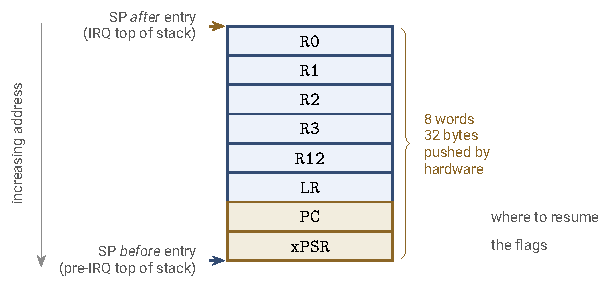
\includegraphics[width=\textwidth]{assets/exception-stack-frame.pdf}
        \end{center}
    \end{column}
    \begin{column}{.36\textwidth}
        {\small
        \begin{itemize}
            \item \texttt{PC} and \texttt{xPSR} make resuming possible:
                  one says \alert{where} to continue, the other restores
                  the flags
            \item Your interrupted code never notices, and needs no
                  special setup code of its own
        \end{itemize}}
    \end{column}
    \end{columns}
\end{frame}

\begin{frame}{You Already Know This: Priority Encoders}
    \leavevmode
\begin{itemize}
	\item Each interrupt request line is an \alert{edge-triggered
		flip-flop}: a peripheral event sets it, and clearing the pending bit
	resets it.
	\item The NVIC examines these pending requests using
	\alert{priority-encoding logic}---the same priority encoder used to
	resolve simultaneous requests.
	\item The winning index selects the corresponding entry in the
	vector table.
\end{itemize}

    \vspace{2mm}
\begin{block}{Why a forgotten pending-flag clear hangs the system}
	If your code never resets that flip-flop, the request remains
	asserted. When the handler returns, the NVIC sees that the line is
	still pending and immediately invokes the handler again. The result
	is
	\alert{an interrupt handler that runs forever}---one of the most
	common interrupt bugs. This is why the handler you already wrote
	contains \texttt{EXTI->PR = (1U \texttt{<}< 13);}.
\end{block}
\end{frame}

\begin{frame}{The NVIC Registers}
    \leavevmode
    {\small You will rarely write these directly, since CMSIS wraps
    them. But it is worth knowing them, since they live at
    \texttt{0xE000E100}:}

	\begin{center}
    {\small
	\striped
	\begin{tabular}{@{}l p{8cm}@{}}
		\toprule
		\textbf{Register} & \textbf{Does} \\
		\midrule
		\texttt{NVIC\_ISER[x]} & Set-enable: writing 1 enables that
		interrupt; writing 0 does nothing \\
		\texttt{NVIC\_ICER[x]} & Clear-enable: writing 1 disables \\
		\texttt{NVIC\_IPR[x]}  & Priority for each channel \\
		\bottomrule
	\end{tabular}}
	\end{center}

    {\small Separate set and clear registers avoid a read-modify-write
    race. \alert{This is the same design idea as GPIO's \texttt{BSRR}}.}
\end{frame}

\begin{frame}[fragile]{Sleeping Between Events}
    \leavevmode
    {\small Once an event is interrupt-driven, the main loop often has
    nothing to do until the next one arrives. \alert{\texttt{WFI}}
    (``wait for interrupt'') lets the CPU stop instead of spinning:}

    \begin{lstlisting}[language=C]
while (1) {
    __WFI();   // sleep until an interrupt wakes the CPU
}
    \end{lstlisting}

    \begin{itemize}
        \item The core's clock halts; the NVIC keeps watching for a
              pending interrupt
        \item On the next interrupt, the core wakes and the usual
              exception entry sequence runs, exactly as if it had been
              running
        \item \textbf{Interrupts} remove the need to \alert{poll} for an
              event; \textbf{\texttt{WFI}} removes the need to
              \alert{keep running} while waiting for one
    \end{itemize}

    \vspace{1mm}
    {\small A battery-powered sensor node can sleep almost all the
    time and wake only when a reading is due.}
\end{frame}

\begin{frame}{Summary}
    \begin{itemize}
        \item \textbf{Polling} wastes the processor and ties response
              time to the loop. \textbf{Interrupts} give a fast, bounded
              response and let the CPU sleep.
        \item On an interrupt, the processor \textbf{automatically}
              pushes eight registers, then restores them on return.
        \item The \textbf{vector table} holds every handler's address,
              and the initial \texttt{SP} in its first word.
        \item A pin reaches the core through \textbf{SYSCFG}
              $\rightarrow$ \textbf{EXTI} $\rightarrow$ \textbf{NVIC}.
              All \texttt{Px}$n$ pins share \texttt{EXTI}$n$, so only
              one may be selected.
        \item In the handler: match the \textbf{name}, \textbf{clear the
              pending flag}, and mark shared variables
              \textbf{\texttt{volatile}}.
        \item \textbf{Keep handlers short.} Set a flag; let
              \texttt{main()} do the real work.
    \end{itemize}

    \vspace{2mm}
    \begin{block}{Next: Chapter 10 --- Timers, Timing and PWM}
        \texttt{delay\_ms()} is wrong in three ways. Next, we learn to do
        timing properly.
    \end{block}
\end{frame}

%===============================================================================
\section{Design Challenge}
%===============================================================================

\begin{frame}{Design Challenge}{To be worked on paper, before any code}
    \leavevmode
    \begin{block}{The brief}
        A system has four event sources: a 1~kHz sensor-ready signal, an emergency-stop button, a 50~Hz zero-crossing detector, and a rotary encoder producing up to 2000 edges per second.
    \end{block}

    \vspace{2mm}
    {\small Decide for each one whether it should be polled or interrupt-driven, and assign interrupt priorities to the ones you choose to interrupt. Justify every decision in terms of latency requirement and service cost. Then identify which pair of sources is most likely to interfere with each other, and state what evidence would tell you the problem had happened.}
\end{frame}

\begin{frame}[plain]
    \begin{center}
        \vfill
        {\usebeamerfont{title}\color{primary}\Huge Questions?}
        \vfill
        {\small\color{Gray} \emph{Introduction to ARM Cortex-M Microprocessors} --- Chapter 9}
        \vfill
    \end{center}
\end{frame}

\end{document}

